%! Author = raquelmolire
%! Date = 25/09/2022

El Alzheimer es una enfermedad neurodegenerativa, progresiva, irreversible y terminal en la que se produce una pérdida
de neuronas principalmente relacionada con dos tipos de alteraciones cerebrales: la acumulación anormal de placas
seniles de proteína beta-amiloide y ovillos neurofibrilares de proteína Tau.

\subsection{Epidemiología de la enfermedad}\label{subsec:epidemiologia}
Es la forma más común de demencia, una pérdida de la función cerebral que afecta la memoria, el pensamiento, el
lenguaje, el juicio y el comportamiento.
Se estima que entre un 60 y un 80 por ciento de los casos de demencia se producen a causa de la EA en los países
desarrollados.

Esta patología tiene una mayor frecuencia en personas mayores de 65 años, siendo la prevalencia de un 7\% en este grupo
de población, y aproximándose al 50\% en mayores de 85 años.
Aunque en otros casos más extremos y mucho menos frecuentes puede ser desarrollada a partir de los 30 años, siendo
denominada en este caso como Enfermedad de Alzheimer precoz o de aparición temprana.
En término medio, una persona con Alzheimer vive de 4 a 8 años después de ser diagnosticada, pero puede vivir hasta 20
años dependiendo de otros factores como es, por ejemplo, la etapa en la que se diagnostique la enfermedad.

Actualmente, en España la cifra de personas afectadas por la enfermedad del Alzheimer es de aproximadamente 1.200.000,
aproximándose a las 5.000.000 personas si contamos con la familia.

\subsection{Cuadro clínico}\label{subsec:cuadro-clinico}
Las lesiones cerebrales características de la EA comienzan años antes de que aparezcan los primeros síntomas, según
concluyen algunas investigaciones, estas alteraciones cerebrales pueden darse entre 10 o 20 años antes.

La EA produce en el cerebro una pérdida neuronal progresiva que se relaciona de manera directa con la acumulación de
placas de proteína beta-amiloide y de ovillos neurofibrilares de proteína Tau que impiden a las neuronas comunicarse
entre sí conduciendo a su muerte.
El conjunto de estas lesiones se inicia en el hipocampo y se distribuye a otras regiones cerebrales según el grado de
evolución de la enfermedad.

El hipocampo es una de las áreas del cerebro cuyo funcionamiento es vital para la memoria y el aprendizaje.
Este es el motivo por el cual, en las primeras etapas de la enfermedad, las personas con EA presentan dificultades para
recordar sucesos recientes o para retener información nueva, sin embargo, se conservan recuerdos del pasado porque las
zonas del cerebro implicadas todavía no se han visto afectadas.

La afectación progresiva de otras áreas cerebrales da lugar a la aparición de otros síntomas que afectan a la toma de
decisiones, cambios conductuales y de personalidad, dificultad para la comunicación y la pérdida de funciones biológicas
que conlleva la muerte.

El desarrollo progresivo de la EA es lo que da lugar a que se establezca una distinción de etapas de la enfermedad según
la evolución de las lesiones en el cerebro y según la evolución de los síntomas que van produciendo esos daños.
Distinguiendo tres etapas: enfermedad de Alzheimer leve (etapa temprana), enfermedad de Alzheimer moderada (etapa media)
y enfermedad de Alzheimer grave (etapa final), las cuales se detallan posteriormente.

\subsection{Cómo afecta al funcionamiento cerebral la acumulación de proteína beta-amiloide y Tau}\label{subsec:acumulacion-proteínas}
La acumulación en el cerebro de placas de proteína beta-amiloide y de ovillos neurofibrilares de proteína Tau provoca la
interrupción de la comunicación, el metabolismo y la reparación de neuronas, que son los procesos que hacen que las
neuronas se mantengan sanas.
La suspensión de estos procesos provoca la muerte de neuronas, y es la que conlleva problemas de memoria.

La proteína beta-amiloide es una proteína presente en el cerebro que lleva a cabo determinadas funciones fisiológicas.
En una persona con EA, la eliminación de los restos de esta proteína no se realiza de manera correcta, provocando la
formación de placas seniles (depósitos extracelulares de beta-amiloide) y afectando al funcionamiento cerebral normal.


La proteína Tau tiene como principal objetivo mantener la estructura de las neuronas.
En personas con EA, se provoca una serie de alteraciones bioquímicas que causan la formación de ovillos neurofibrilares
como un conglomerado anormal de proteínas que se compone de pequeñas fibrillas entrelazadas en el interior de las
neuronas.

A medida que las neuronas mueren y las conexiones entre las redes de neuronas se rompen, muchas regiones del cerebro
comienzan a encogerse.
En la etapa final de la EA, el daño cerebral producido es muy grande, resultando una pérdida significativa del volumen
de tejido cerebral.

\begin{figure}[H]
    \centering
    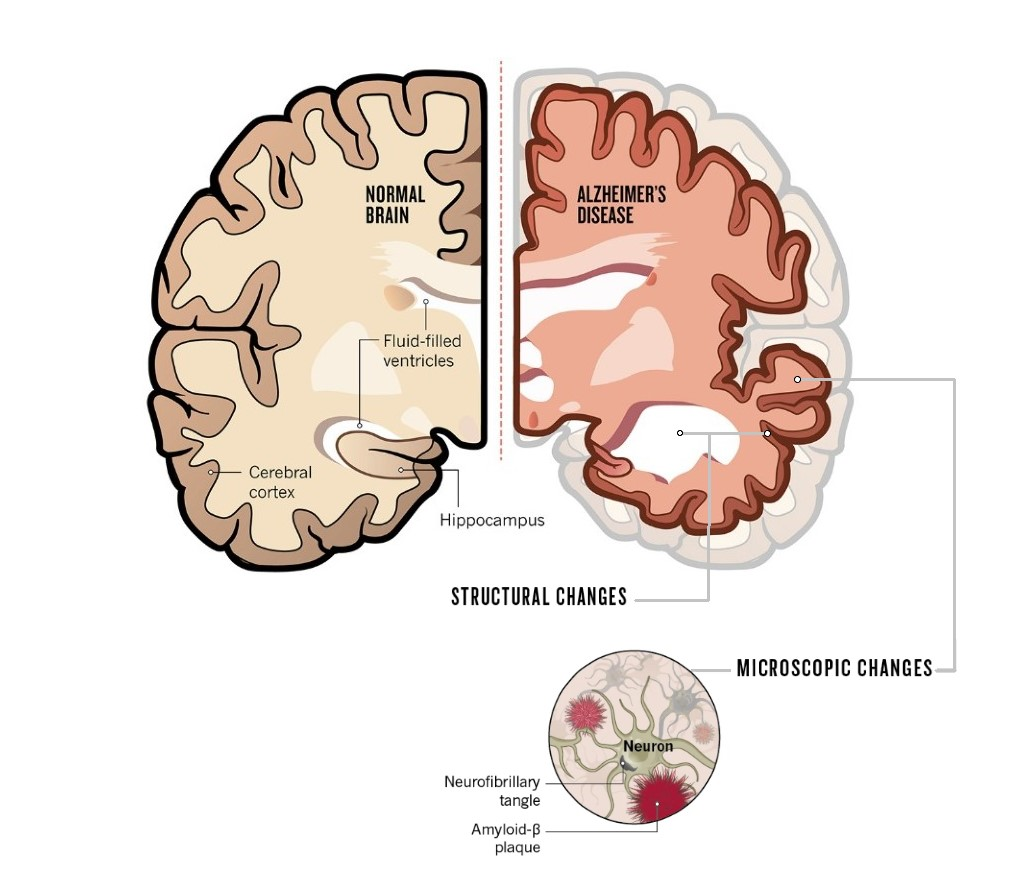
\includegraphics[width=\textwidth]{./imgs/lesiones-cerebrales}
    \caption{Lesiones cerebrales producidas por la enfermedad de Alzheimer.\\Imagen adaptada de una
    ilustración de Stacy Jannis, Alzheimer\'s Association.}
    \label{fig:lesiones-cerebrales}
\end{figure}

\subsection{Fases de la enfermedad}\label{subsec:fases-enfermedad}
La EA es una enfermedad de larga evolución en la que, usando una escala de clasificación común, se distinguen tres fases.

\subsubsection{Enfermedad de Alzheimer leve (etapa temprana)}\label{subsubsec:etapa-temprana-EA}
Esta etapa permite al paciente desenvolverse de forma independiente, pero aparecen los fallos de memoria, como son:
\begin{itemize}
    \item Dificultad para encontrar la palabra o el nombre correctos.
    \item Problemas para realizar tareas en entornos sociales o laborales, destacando la presencia de cambios de
    personalidad.
    \item Olvidarse de algo que acaba de leer.
    \item Problemas para encontrar objetos.
    \item Dificultad para recordar acontecimientos y conversaciones recientes.\\
\end{itemize}

Realizar un diagnóstico de la enfermedad en esta etapa puede ser determinante, ya que existe la posibilidad de aplicar
tratamientos con los que la evolución de la enfermedad pueda ralentizarse sin que resulten perjudiciales para la salud
del paciente.
Sin embargo, es muy difícil realizar el diagnóstico en esta fase pues la mayoría de los síntomas se suelen confundir con
conductas características de la vejez.

\subsubsection{Enfermedad de Alzheimer moderada (etapa media)}\label{subsubsec:etapa-media-EA}
En esta etapa comienzan las limitaciones en las actividades de la vida diaria y la persona con EA necesita un nivel de
atención mayor en tareas básicas como la alimentación o el aseo personal.

La memoria se sigue viendo afectada, de manera más pronunciada en esta etapa, como puede ser dificultad para reconocer a
miembros de la familia, olvidarse eventos o información de la historia personal, o el aumento del riesgo de
desorientarse y perderse en lugares conocidos.

\subsubsection{Enfermedad de Alzheimer grave (etapa final)}\label{subsubsec:etapa-final-EA}
En esta etapa las personas con EA pierden la capacidad de responder a su entorno, sufriendo una pérdida completa de la
memoria y las capacidades intelectuales y funcionales.
Provocando la necesidad de cuidado y asistencia absoluta.
Se produce una pérdida progresiva del lenguaje haciendo que el paciente deje de hablar y una posterior inmovilidad
completa.

La pérdida de las capacidades funcionales hace que se produzca una pérdida de peso y disminución de sus defensas
inmunológicas que conllevan a la muerte.

\subsection{Diagnóstico de la enfermedad}\label{subsec:diagnostico-enfermedad}
Para diagnosticar la EA se requiere de evaluaciones médicas exhaustivas, en las que se evalúa el deterioro de la memoria,
la presencia de cambios de conducta y el estado de otras habilidades de razonamiento, que permitan determinar cuáles son
las capacidades funcionales.
Además, es necesario realizar pruebas médicas que descarten otras posibles causas de deterioro.

El diagnóstico se puede dividir en cuatro partes:
\begin{itemize}
    \item Evaluación del estado mental: Se evalúan las habilidades de razonamiento (cognitivas) y memoria.
    \item Examen físico: Se evalúa la salud general de la persona, para descartar otras afecciones tratables que causen
    síntomas similares.
    \item Examen neurológico: Se realiza una evaluación de afecciones cerebrales y de salud mental, descartando algún
    trastorno como la depresión.
    \item Pruebas de laboratorio y estudios de imágenes cerebrales.\\
\end{itemize}

\subsubsection{Pruebas de laboratorio}\label{subsubsec:pruebas-laboratorio-EA}
Las pruebas de laboratorio incluyen: análisis de sangre para descartar otros trastornos, o examen del líquido
cefalorraquídeo para medir los niveles de proteína amiloide y tau, determinando según su proporción si se trata de EA.
Los exámenes del líquido cefalorraquídeo solo se realizan en casos atípicos y de rápida evolución.

\subsubsection{Pruebas de diagnóstico por imágenes}\label{subsubsec:pruebas-imagenes-EA}
Las pruebas de diagnóstico por imágenes ayudan a distinguir diferentes tipos de enfermedades cerebrales degenerativas y
además establecer cuál es el grado de degeneración, por lo que son las pruebas más fiables para el diagnóstico del
Alzheimer.

Las técnicas más frecuentes de diagnóstico por imágenes son:
\begin{itemize}
    \item Imagen por Resonancia Magnética (MRI): Es una técnica no invasiva que a través de campos magnéticos genera imágenes
    anatómicas tridimensionales.
    Proporciona información exhaustiva de los tejidos blandos y permite examinar la anatomía del cerebro y evaluar
    lesiones presentes.
    \item Tomografía Computarizada (más conocida como TAC): Con esta técnica se recopilan imágenes transversales
    sucesivas mediante rayos X. Proporciona imágenes óseas, de tejidos blandos y aire y permite identificar anomalías
    asociadas al Alzheimer.
    \item Tomografía por emisión de positrones (PET): Esta técnica usa radiofármacos de administración intravenosa
    gracias a los cuales se obtienen imágenes de alta definición en las que se pueden detectar y visualizar depósitos
    extracelulares de proteína beta-amiloide.\\
\end{itemize}

\begin{figure}[H]
    \centering
    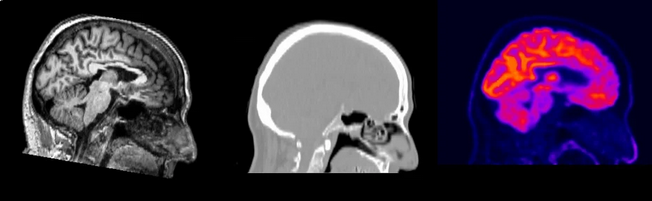
\includegraphics[width=\textwidth]{./imgs/MRI-TAC-PET}
    \caption{Técnicas de diagnóstico por imágenes de la enfermedad de Alzheimer.\\ De izquierda a derecha: MRI, TAC y PET.
    \\Fuente: Biotechnology portal in Spain.}
    \label{fig:tecnicas-diagnosico-imagen}
\end{figure}